\chapter{Pendahuluan} \label{ch:chapter_1}

\section{Latar Belakang}

Badan Pusat Statistik (BPS) merupakan suatu lembaga pemerintah non-departemen yang bertanggung jawab dalam penyediaan statistik dasar \citep{bps_badan_2016}. Dalam peranannya sebagai penyedia data, BPS melakukan pengumpulan data dengan 2 (dua) metode, yaitu primer dan sekunder. Pengumpulan data primer adalah pengumpulan data dengan menggunakan metode wawancara langsung dengan responden, baik responden individu, rumah tangga, maupun perusahaan. Sementara pengumpulan data sekunder adalah pengumpulan data dengan memanfaatkan data yang telah dikumpulkan oleh pihak lain.


Pada pengumpulan data primer oleh BPS, selanjutnya disebut dengan pencacahan, suatu wilayah administratif dibagi dalam beberapa Blok Sensus (BS). Blok sensus merupakan wilayah kerja dari seorang pencacah \citep{bps_sistem_2016}. Setiap petugas pengumpulan data, disebut dengan pencacah, akan dialokasikan dalam beberapa blok sensus yang akan menjadi tanggung jawabnya. Pencacah kemudian akan mendatangi blok sensus tersebut dan mengunjugi setiap rumah tangga yang menjadi sampel pencacahan.


\begin{figure}[h]
    \centering
    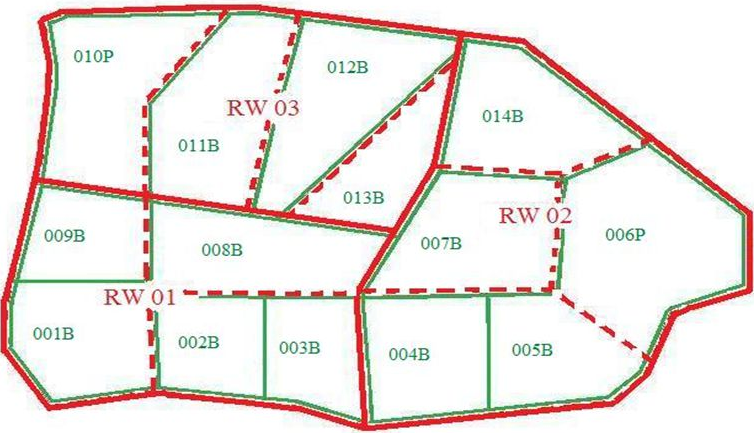
\includegraphics[width=10cm]{../../Resources/Images/peta_kelurahan_per_bs}
    \caption{Pembagian Blok Sensus dalam Desa/Kelurahan}
    \label{fig:capi-ilustration}
\end{figure}


Pengalokasian pencacah terhadap blok sensus terkadang menjadi sesuatu yang sulit, karena terkait dengan waktu dan biaya. \textit{Subject matter} yang menangani kegiatan harus mempertimbangkan beberapa hal, salah satunya adalah jarak antar blok sensus yang menjadi wilayah kerja seorang pencacah. Kesalahan dalam pengalokasian blok sensus menyebabkan waktu pencacahan menjadi lama, yang dapat mempengaruhi kegiatan pencacahan secara keseluruhan.


Selain jarak antar blok sensus, faktor yang juga perlu diperhatikan adalah lamanya pencacahan dalam sebuah blok sensus. Lama pencacahan dalam blok sensus secara umum dipengaruhi oleh 2 (dua) faktor, jarak antar rumah tangga dalam suatu blok sensus dan lama wawancara dalam rumah tangga. \citep{sudman_time_1965}, dalam penelitiannya menyatakan bahwa mengunjungi sebuah segmen dapat menghabiskan 21 persen dari keseluruhan waktu, 15 persen untuk mengunjungi rumah tangga dalam sebuah segmen, 37 persen untuk wawancara, dan sisanya untuk kegiatan lain, seperti \textit{editing}, \textit{study}, dan \textit{clerical}.


Faktor-faktor yang terkait dengan alokasi blok sensus dan petugas tersebut diatas, seperti: jarak antar blok sensus, jarak antar rumah tangga, dan lama wawancara tidaklah selalu tersedia. Andaikan tersedia, datanya-pun bersifat relatif, seperti lama wawancara yang sangat tergantung pada kemampuan pencacah dalam bertanya dan menggali jawaban, tingkat pendidikan responden, dan banyaknya anggota rumah tangga yang harus didata. Oleh karena itu diperlukan suatu cara atau metode yang memungkinkan pengalokasian petugas terhadap blok sensus secara dinamis sesuai dengan context.


Dalam sistem komputer tidak terdapat definisi \textit{context} yang tunggal. Meskipun demikian, sebagian besar definisi sepakat bahwasannya \textit{context} adalah sesuatu yang harus dilakukan terkait interaksi pengguna dan sistem komputer \citep{chen_survey_2000}. \citep{schilit_context-aware_1994}, misalnya, membagi \textit{context} menjadi 4 (empat): \textit{computing context}, \textit{user context}, \textit{physical context}, dan \textit{time context}. \textit{Computing context} meliputi: \textit{network connectivity}, \textit{communication cost}, \textit{communication bandwidth}, dan \textit{nearby resource}; \textit{user context} meliputi: \textit{user profile}, \textit{location}, dan \textit{social situation}; \textit{physical context} meliputi: \textit{lighting}, \textit{noise}, \textit{traffic condition}, dan \textit{temperature}; serta \textit{time context} meliputi: \textit{time of a day}, \textit{week}, \textit{month} and \textit{season of the year}. Senada dengan \citep{schilit_context-aware_1994}, \citep{schmidt_there_1999} mendefinisikan \textit{context} sebagai pengetahuan tentang \textit{state} dari \textit{user} dan \textit{IT device}, termasuk lingkungan, situasi, dan lokasi. Sementara \citep{abowd_towards_1999} mendefinisikan \textit{context} sebagai segala informasi yang dapat digunakan untuk mengkarakterisasi kondisi dari suatu entitas. Entitas yang dimaksud dapat berupa manusia, tempat atau obyek yang relevan dengan aplikasi dan pengguna, termasuk aplikasi dan pengguna itu sendiri. 


\begin{figure}[h]
    \centering
    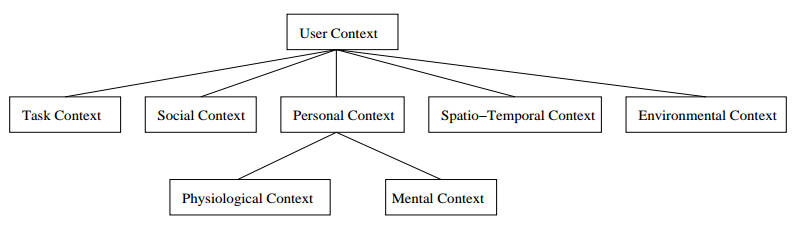
\includegraphics[width=\textwidth]{../../Resources/Images/context}
    \caption{Context Hierarchy \citep{kofod-petersen_case-based_2003}}
    \label{fig:capi-ilustration}
\end{figure}


\textit{Context-aware application} telah banyak digunakan di berbagai bidang. \citep{tsai_context-aware_2016} misalnya, menggunakan \textit{context} untuk menciptakan \textit{smart home environment}. \citep{magara_mplist:_2016} menggabungkan beberapa \textit{context} seperti: lokasi dan aktivitas pengguna, preferensi, label, dan \textit{tags} untuk membuat rekomendasi musik yang akan diputar. Sementara \citep{said_introduction_2013} menciptakan rekomendasi film berdasarkan \textit{time}, \textit{mood}, dan \textit{social recommendation}.


Pada aplikasi yang bersifat \textit{mobile}, \textit{context} biasanya diperoleh dengan menggunakan sensor yang tersemat dalam \textit{mobile device} tersebut. Sekarang ini, telah banyak ditemui \textit{mobile device}, terutama \textit{programmable smartphone}, yang telah dilengkapi dengan berbagai sensor \citep{cao_mobile_2015}. \citep{do_groupus:_2011}, misalnya mem-\textit{propose} GroupUs, framework yang mengelompokkan pengguna berdasarkan aktifitas sehari-hari yang dikumpulkan dengan menggunakan \textit{proximity sensor}. \citep{dai_mobile_2010} menciptakan \textit{drunk driving detection} dengan memanfaatkan sensor \textit{accelerometer} yang tersemat dalam \textit{smartphone}. Sementara \citep{zou_context-aware_2016}, memanfaatkan sensor \textit{Global Posisioning System} (GPS) dan \textit{Micro-Electro-Mechanical System} (MEMS) untuk membuat rekomendasi transportasi. Begitu pula sensor-sensor yang lain juga telah dimanfaatkan dalam berbagai penelitian \citep{dai_perfalld:_2010, lu_soundsense:_2009, bao_movi:_2010, rubel_toward_2005, atzmueller_towards_2013}.


Di sisi yang lain, \textit{location recommendation} merupakan sebuah bahasan yang juga banyak diteliti. Metode yang banyak digunakan untuk menentukan rekomendasi lokasi adalah \textit{Location-based Social Network} (LBSN). Cara kerja LBSN pada dasarnya adalah dengan memanfaatkan lokasi dan \textit{point of interest} yang dibagikan oleh pengguna \citep{yuan_location_2016}. Beberapa peneliti juga mencoba meningkatkan akurasi prediksi dengan menggabungkannya dengan berbagai metode. Misalnya \citep{koren_collaborative_2010}, menggunakan \textit{temporal factorization model} yang memberikan hasil lebih baik dibanding dengan \textit{non-temporal factorization model}. Sementara  \citep{pragarauskas_temporal_2010} mengadopsi \textit{bayesian probabilistic tensor factorization} untuk mewujudkan \textit{temporal collaborative filtering}. Akan tetapi, metode LBSN tidak sesuai digunakan untuk membuat rekomendasi lokasi pencacahan. Hal ini dikarenakan metode LBSN menggunakan \textit{logs} yang telah dikumpulkan sebelumnya, baik \textit{location logs} maupun \textit{user preference logs}, untuk menentukan rekomendasi, sementara lokasi pencacahan bukan merupakan \textit{point of interest} yang dikunjungi oleh banyak orang.


Metode lain yang juga banyak digunakan adalah \textit{Travelling Salesman Problem} (TSP). TSP adalah sebuah algoritma klasik \citep{biggs_graph_1976} yang telah banyak diadopsi dan dimodifikasi. Masalah yang umumnya mejadi dasar modifikasi adalah penggunaan \textit{multiple salesman}, yang disebut dengan \textit{Multiple Travelling Salesman Problem} (MTSP) \citep{bektas_multiple_2006}. Variasi dari MTSP juga telah banyak diteliti, yang umumnya mencakup: \textit{single or multiple depots} (\textit{start and stop point}), jumlah \textit{salesman}, \textit{fixed charges} (jika jumlah \textit{salesman} tidak tetap), lama kunjungan (\textit{time window}), dan \textit{special restrictions} \citep{bektas_multiple_2006}. Berbagai aplikasi untuk menyelesaikan permasalahan nyata (\textit{real-life problem}) juga telah dikembangkan dengan menggunakan MTSP. Misalnya, \textit{print press scheduling} oleh \citep{gorenstein_printing_1970}, \textit{crew scheduling} oleh \citep{svestka_computational_1973}, \textit{school bus routing problem} oleh \citep{angel_computer-assisted_1972}, \textit{interview scheduling} oleh \citep{gilbert_new_1992}, \textit{mission planning} oleh \citep{brumitt_dynamic_1996}, \textit{hot rolling scheduling} oleh \citep{tang_multiple_2000}, dan \textit{global navigation satellite system surveying networks} oleh \citep{saleh_design_2004}.


\begin{figure}[h]
    \centering
    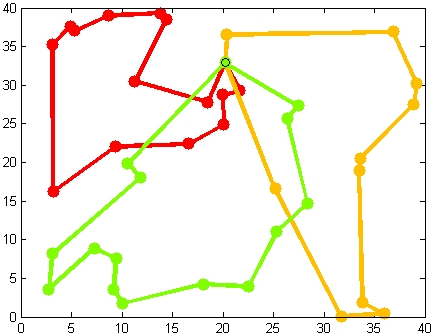
\includegraphics[width=10cm]{../../Resources/Images/mtsp}
    \caption{Ilustrasi \textit{Multiple Travelling Salesman Problem}}
    \label{fig:mtsp-ilustration}
\end{figure}


Asumsi yang digunakan dalam pendekatan MTSP adalah semua informasi telah tersedia pada saat perancangan. Sementara dalam pencacahan informasi tidak selalu tersedia. Misalnya, \textit{time windows}, yang tersusun atas jarak antar rumah tangga dan lama wawancara, merupakan variabel yang bersifat dinamis. Jarak antar rumah tangga sangat tergantung dari sampel yang terpilih, sementara lama wawancara sangat tergantung dari kemampuan pencacah dalam bertanya dan menggali jawaban, tingkat pendidikan responden, dan banyaknya anggota rumah tangga yang harus didata. Untuk itu, diperlukan suatu cara agar metode MTSP dapat mengakomodir \textit{time windows} secara dinamis.


Solusi yang ditawarkan adalah dengan mengabaikan \textit{time windows}, kemudian meng-\textit{generate} rekomendasi baru setiap kali pencacah telah menyelesaikan pencacahan pada suatu blok sensus. Untuk mencegah blok sensus yang telah dicacah diikutsertakan dalam rekomendasi, maka akan digunakan \textit{tabu search}. \textit{Tabu search} dirancang oleh \citep{glover_tabu_1989, glover_tabu_1990} untuk menyelesaikan masalah optimasi kombinasi, yang aplikasinya berkisar dari \textit{graph theory} dan \textit{matroid settings} untuk masalah pemrograman integer. \textit{Tabu search} menggunakan \textit{tabu list}, yaitu suatu struktur data yang menyimpan semua solusi yang telah dikunjungi sebelumnya \citep{orourke_dynamic_1999}. Untuk menyusun \textit{tabu list}, maka dalam kasus ini akan digunakan metode \textit{publish-subscribe}, atau biasa disingkat dengan pub-sub. Metode pub-sub yang akan digunakan adalah pub-sub \textit{tracking service}, sebagaimana diusulkan oleh \citep{chen_efficient_2003}.


\section{Rumusan Masalah}

Berdasarkan latar belakang permasalahan yang telah diuraikan sebelumnya, dan didasari motivasi untuk menciptakan rekomendasi alokasi pencacah dan blok sensus secara dinamis, maka dapat dirumuskan masalah dalam penelitian ini adalah bagaimana merancang sebuah sistem rekomendasi lokasi pencacahan dengan memanfaatkan \textit{context} dari pencacah.


Adapun detail dari permasalahan yang akan dikaji adalah sebagai berikut:

\begin{itemize}
\item Bagaimana menentukan \textit{context} apa saja yang dapat digunakan dalam kasus ini.
\item Bagaimana membuat rekomendasi lokasi pencacahan pada kondisi \textit{time windows} sangat berpengaruh, tetapi data tidak tersedia.
\item Bagaimana membuat \textit{conflict resolution}, agar dua atau lebih \textit{smartphone} tidak merekomendasikan lokasi yang sama.
\end{itemize}


\section{Tujuan Penelitian}

Berdasarkan rumusan masalah diatas, maka dapat ditentukan tujuan utama dari penelitian ini adalah untuk menciptakan sebuah sistem rekomendasi lokasi pencacahan secara dinamis. 

Adapun tujuan khusus dari penelitian ini adalah:

\begin{itemize}
\item Mengidentifikasi \textit{context} yang terkait dengan penentuan lokasi pencacahan.
\item Menyusun algoritma rekomendasi.
\item Menyusun algoritma \textit{location conflict}.
\item Mengimplementasikan algoritma usulan dalam \textit{mobile application}.
\item Melakukan ujicoba algoritma dan aplikasi usulan.
\end{itemize}


\section{Batasan Masalah}

Masalah dalam penelitian ini memiliki batasan sebagai berikut:

\begin{itemize}
\item Lokasi pencacahan yang menjadi rujukan adalah Blok Sensus (BS) yang dikeluarkan oleh Badan Pusat Statistik (BPS).
\item \textit{Device} yang digunakan adalah \textit{smartphone} berbasis Android yang umum dijual dipasaran.
\item Tidak mempertimbangkan lingkungan yang tidak terkoneksi dengan jaringan komunikasi.
\end{itemize}


\section{Implikasi}

Manfaat yang dapat diperoleh dari penelitian ini antara lain:


\section{Sistematika Penulisan}

Sistematika penulisan tesis ini terdiri atas enam bab dengan perincian sebagai berikut:

